\documentclass[10pt,twocolumn,letterpaper]{article}

\usepackage{iccv}
\usepackage{times}
\usepackage{epsfig}
\usepackage{graphicx}
\usepackage{amsmath}
\usepackage{amssymb}
\usepackage{booktabs}
\usepackage{subcaption}
\usepackage{multirow}
\usepackage[breaklinks=true,bookmarks=false]{hyperref}

\iccvfinalcopy

\ificcvfinal\pagestyle{empty}\fi

\begin{document}

\title{Spatiotemporal Relighting in 4D Gaussian Splatting}

\author{Ranveer Singh \and Shreyas Garimella\\
Princeton University\\
Department of Computer Science\\
COS 526: Neural Rendering\\
{\tt\small \{sg610, ku6042\}@princeton.edu}
}

\maketitle
\ificcvfinal\thispagestyle{empty}\fi

%%%%%%%%% ABSTRACT
\begin{abstract}
We present a pipeline for harmonizing the lighting of composite objects within 4D Gaussian Splatting (4DGS) scenes. While compositing objects into static 3D Gaussian scenes is straightforward through point cloud merging, 4D scenes present additional challenges due to temporal deformation and the entanglement of appearance information within spherical harmonic (SH) coefficients. Our method optimizes the SH coefficients of transplanted objects via backpropagation through a differentiable rasterizer, using either a pretrained image harmonization network or paired ground-truth renders as supervision. We evaluate our approach on synthetic Blender scenes with controlled lighting conditions and also explore using DiFix3D+ for per-frame artifact cleanup on real-world HyperNeRF composites. Our experiments reveal that restricting optimization to the DC (zeroth-order) SH band produces clean, artifact-free relighting, while optimizing all SH bands introduces rainbow artifacts from overfitting view-dependent color. We also compare against TranSplat's closed-form SH transfer and show that our optimization-based approach outperforms it by 1.1 dB PSNR on the controlled Blender benchmark.
\end{abstract}

%%%%%%%%% INTRODUCTION
\section{Introduction}

The ability to compose and edit dynamic 3D scenes is becoming increasingly important for applications in augmented reality, film production, and simulation. 3D Gaussian Splatting (3DGS)~\cite{kerbl3Dgaussians} has recently emerged as a fast, explicit alternative to Neural Radiance Fields (NeRF)~\cite{mildenhall2020nerf} for novel view synthesis, offering real-time rendering while maintaining high visual fidelity. Its extension to dynamic scenes, 4D Gaussian Splatting (4DGS)~\cite{wu20244dgaussiansplattingrealtime}, adds a time-conditioned deformation network that warps Gaussians across timesteps, enabling reconstruction from multi-view video.

A natural operation in scene editing is object compositing: inserting an object reconstructed in one environment into a scene captured under different lighting. In 3DGS, this can be done by merging point clouds, but the result often exhibits visible lighting inconsistencies because each Gaussian's appearance is encoded in its spherical harmonic (SH) coefficients, which bake in the illumination from the original capture. In 4DGS, this problem is compounded by the deformation network, which entangles motion with appearance.

Prior work on relighting 3D Gaussians has focused on decomposing materials and illumination~\cite{gao2023relightable3dgaussian}, but these methods require specialized training procedures and do not extend to the 4DGS setting. TranSplat~\cite{chen2024transsplat} proposes a closed-form SH coefficient transfer using environment map ratios, but assumes clean separation between material and lighting in the SH representation, an assumption that does not hold for 4DGS-trained models.

To account for there being no clean separation between material and lighting for 4D Gaussians, as well as the challenge of maintaining consistency across time in 4DGS, we propose a gradient-based optimization pipeline that adjusts the SH coefficients of a masked subset of Gaussians to match target renders produced by an image harmonization network. Our key finding is that restricting optimization to the DC (zeroth-order) SH band avoids the rainbow artifacts that arise from overfitting higher-order view-dependent terms, while still achieving meaningful relighting. We validate our approach on a custom Blender benchmark with paired lighting conditions.

Our contributions are:
\begin{itemize}
\item A differentiable SH optimization pipeline for relighting composited objects in 4DGS scenes, compatible with both static and dynamic deformation.
\item A synthetic Blender benchmark with extreme lighting differences between background and foreground for quantitative evaluation of 4DGS harmonization.
\item An analysis of SH band sensitivity showing that DC-only optimization is preferable to full-band optimization for relighting.
\item A comparison against TranSplat's closed-form SH transfer, demonstrating a 1.1 dB improvement in PSNR.
\end{itemize}

%%%%%%%%% RELATED WORK
\section{Related Work}

\paragraph{3D and 4D Gaussian Splatting.}
3DGS~\cite{kerbl3Dgaussians} represents scenes as collections of 3D Gaussians, each parameterized by position, covariance, opacity, and SH color coefficients. Rendering proceeds via differentiable splatting and alpha compositing, enabling gradient-based optimization from multi-view images. 4DGS~\cite{wu20244dgaussiansplattingrealtime} extends this to dynamic scenes by introducing a deformation field based on HexPlane~\cite{fridovich2023kplanes} representations that predicts per-Gaussian position, rotation, and scale offsets conditioned on time.

\paragraph{Relighting in Gaussian Representations.}
Relightable 3DGS~\cite{gao2023relightable3dgaussian} decomposes Gaussians into BRDF parameters and uses ray tracing for relighting, but requires specialized training and does not support 4DGS deformation. TranSplat~\cite{chen2024transsplat} performs closed-form SH coefficient transfer by computing the ratio between source and target environment maps projected onto the SH basis. However, this approach assumes that SH coefficients cleanly encode lighting, which breaks for 4DGS models where SH coefficients absorb training artifacts, geometric failures, and deformation residuals.

\paragraph{Image Harmonization.}
Image harmonization adjusts the appearance of a composited foreground region so that it looks visually consistent with the surrounding background. These methods do not explicitly model illumination or perform physics-based relighting; instead, they learn statistical priors for color and tone consistency from large datasets of composites. The Whitebox Harmonizer~\cite{ke2022harmonizer} predicts a sequence of global image filters (color temperature, brightness, contrast, saturation) applied to the foreground. PCT-Net~\cite{guerreiro2023pctnet} learns per-pixel color transforms via a CNN backbone. Both take a composite image and foreground mask as input and produce a corrected 2D image. We use them as target generators whose outputs are distilled back into 3D SH coefficients by our optimization pipeline.

\paragraph{Scene Segmentation.}
Segment Any 4D Gaussians (SA4D)~\cite{ji2024segment4dgaussians} extends SAM~\cite{kirillov2023sam} to 4DGS by training a per-Gaussian segmentation network, enabling interactive selection of objects for editing. We build on this framework and use its segmentation masks to identify which Gaussians to harmonize. This mask ensures the backpropagation only updates the SH coefficients for the composited object and not the entire scene.

%%%%%%%%% METHOD
\section{Method}

\subsection{Problem Formulation}

Given a 4DGS scene containing a composited object with mismatched lighting, our goal is to adjust the SH coefficients of the object's Gaussians so that the rendered appearance matches the background scene's lighting conditions. Let $\mathcal{G} = \{(\mu_i, \Sigma_i, \alpha_i, \mathbf{f}_i)\}_{i=1}^N$ denote the set of Gaussians, where $\mu_i$ is position, $\Sigma_i$ is covariance, $\alpha_i$ is opacity, and $\mathbf{f}_i \in \mathbb{R}^{48}$ contains the SH coefficients (up to degree 3, with 16 coefficients per RGB channel). Let $\mathcal{M} \subset \{1, \ldots, N\}$ be the set of indices identifying the Gaussians that belong to the composited object whose lighting we want to correct.

We optimize a per-Gaussian residual $\Delta\mathbf{f}_i$ for $i \in \mathcal{M}$, added to the original SH coefficients before rendering. The rendering function $R(\mathcal{G}, c, t)$ produces an image given camera $c$ and time $t$ via the differentiable rasterizer with deformation applied.

Our pipeline has three stages: (1)~for each training view, render the composite scene and run a 2D harmonizer CNN on the rendered image to produce a target image showing what the object \textit{should} look like under the correct lighting; (2)~re-render the scene with learnable SH residuals and compute the loss between this render and the harmonizer's target, masked to the object region; (3)~backpropagate through the differentiable rasterizer to update only the SH residuals. After convergence, the residuals are baked into the Gaussians and saved as a new PLY file.

\subsection{Target Generation}

For each training view $(c_j, t_j)$, we render the composite scene to produce image $I_j = R(\mathcal{G}, c_j, t_j)$. We also render a 2D mask $M_j$ by rasterizing the 3D Gaussian mask through the same pipeline. The target image $\hat{I}_j$ is obtained by one of two methods:

\begin{enumerate}
\item \textbf{Harmonizer CNN}: A pretrained image harmonization network takes $(I_j, M_j)$ and produces a harmonized output where the masked region's appearance matches the background lighting. We support two backends: the Whitebox Harmonizer~\cite{ke2022harmonizer}, which decomposes corrections into interpretable filter steps, and PCT-Net~\cite{guerreiro2023pctnet}, which learns pixel-wise color transforms.
\item \textbf{Scene B ground truth}: For controlled experiments, we render a paired scene with correct lighting and use those images directly as targets.
\end{enumerate}

\subsection{SH Optimization}

We minimize the loss over all training views:
\begin{equation}
\mathcal{L} = \sum_j \left[ \lambda_1 \| (R_j' - \hat{I}_j) \odot M_j \|_1 + \lambda_2 \mathcal{L}_{\text{reg}} \right]
\label{eq:loss}
\end{equation}
where $R_j' = R(\mathcal{G}', c_j, t_j)$ is the render with modified Gaussians $\mathcal{G}' = \mathcal{G} + \Delta\mathbf{f}$, and $\mathcal{L}_{\text{reg}} = \|\Delta\mathbf{f}\|_2^2$ regularizes the residuals toward zero.

Gradients flow through the differentiable rasterizer to update only $\Delta\mathbf{f}$ for masked Gaussians. All other parameters, including positions, covariances, opacities, and the deformation network, are frozen. Freezing the deformation network is critical: if it were allowed to update, the optimizer could alter the object's motion or shape to reduce the color loss rather than correcting the SH coefficients, destroying the original temporal dynamics of the scene.

\subsection{DC-Only Optimization}
\label{sec:dconly}

The SH basis decomposes color into bands of increasing angular frequency. The zeroth-order (DC) coefficient represents the view-independent base color (radiance), while bands $l=1,2,3$ encode view-dependent effects such as specular highlights that shift with viewing angle. A lighting change such as moving an object from a dark forest to a bright garden primarily affects the overall brightness and color temperature, which are captured entirely by the DC coefficient.

We found that optimizing all 16 SH coefficients per channel with uniform learning rates leads to severe rainbow and iridescent artifacts. The optimizer exploits higher-order bands to minimize loss at specific training viewpoints, creating view-dependent color patterns that fail to generalize to novel perspectives. In the 4DGS framework, these artifacts warp inconsistently over time as the underlying geometry deforms. As illustrated in Table~\ref{tab:sh_deltas}, higher-frequency bands receive updates 3$\times$ larger than the DC component; this imbalance is physically counter-intuitive, as relighting is fundamentally a low-frequency operation that should be dominated by the zeroth-order term.

Our recommended configuration sets the learning rate for DC to 0.01 and freezes all higher bands ($\text{lr}_{\text{rest}} = 0$). This produces clean, uniform color shifts without view-dependent artifacts.

\begin{table}[t]
\centering
\small
\begin{tabular}{lcc}
\toprule
SH Band & Mean $|\Delta|$ & Max $|\Delta|$ \\
\midrule
DC ($l=0$) & 0.032 & 1.28 \\
$l=1$ & 0.090 & 2.05 \\
$l=2$ & 0.096 & 2.24 \\
$l=3$ & 0.105 & 2.26 \\
\bottomrule
\end{tabular}
\caption{Mean and maximum absolute SH residuals per band when optimizing all bands equally. Higher bands receive disproportionately large updates relative to DC, causing view-dependent color artifacts.}
\label{tab:sh_deltas}
\end{table}

%%%%%%%%% EXPERIMENTS
\section{Experiments}

\subsection{Synthetic Blender Benchmark}

\paragraph{Scene Construction.}

An issue that we repeatedly ran into was that there were no existing 4DGS benchmarks that provided paired scenes with extreme mismatched lighting differences. We constructed a synthetic benchmark in Blender consisting of two animated characters (a breakdancing mannequin and a stylized cat) placed in a snowy outdoor environment. Two HDR environment maps provide the lighting conditions: \textit{suburban\_garden} (bright, diffuse outdoor light) and \textit{forest} (dark, warm light with dappled shadows).

\textbf{Scene A} (mismatched): The cat is rendered under forest lighting while the breakdancer and background use suburban garden lighting. After compositing, the cat appears too dark relative to its surroundings. \textbf{Scene B} (ground truth): Both objects and the background are rendered under suburban garden lighting. Figure~\ref{fig:blender_scenes} shows the two scenes from the same camera pose.

In Blender, we render 200 training views and 40 test views at 800$\times$800 resolution across a 100-degree azimuth arc at three elevation levels, following the D-NeRF~\cite{pumarola2021dnerf} dataset format. For dynamic scenes, the breakdancer performs a 75-frame animation at 0.3$\times$ speed, giving approximately 5 views per timestep. All scenes are trained with 4DGS using 50K iterations.

\begin{figure}[t]
\centering
\begin{subfigure}{0.48\linewidth}
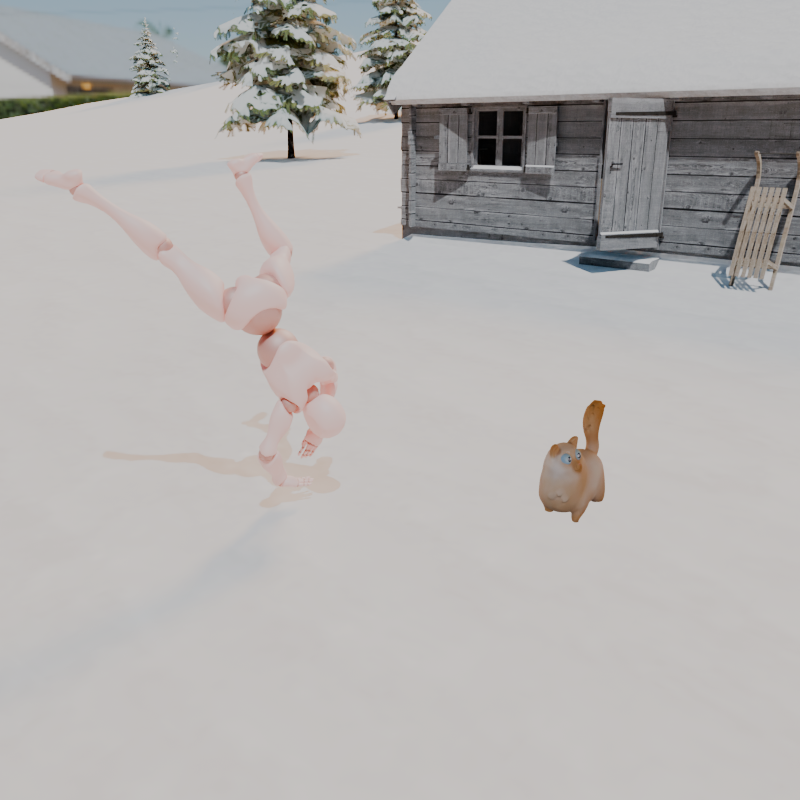
\includegraphics[width=\linewidth]{figures/blender_scene_a.png}
\caption{Scene A (mismatched)}
\end{subfigure}
\hfill
\begin{subfigure}{0.48\linewidth}
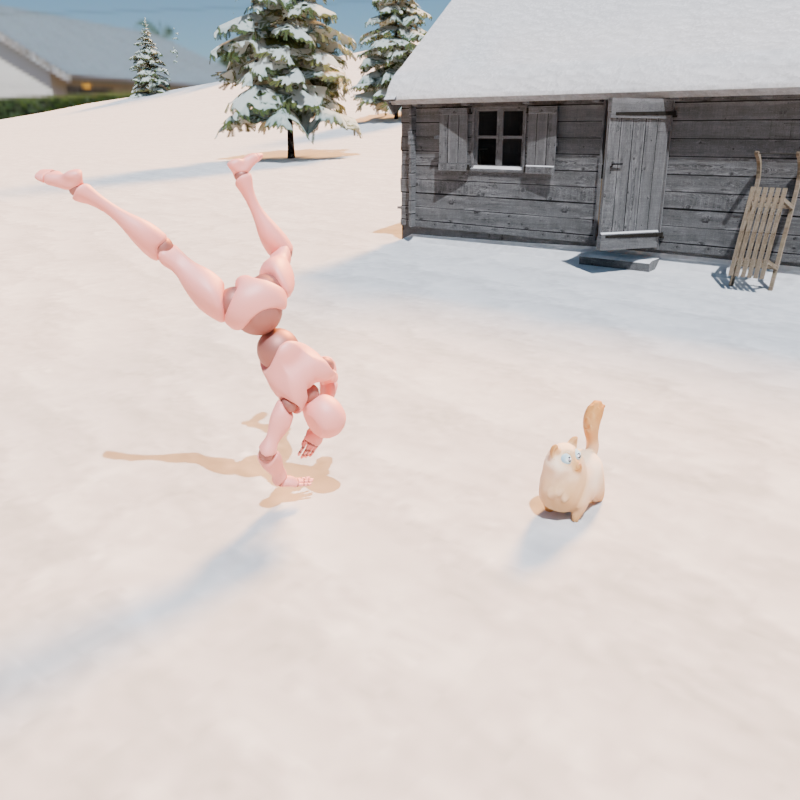
\includegraphics[width=\linewidth]{figures/blender_scene_b.png}
\caption{Scene B (ground truth)}
\end{subfigure}
\caption{Blender benchmark scenes. In Scene A, the cat is rendered under dark forest lighting then composited onto the suburban garden background, creating a visible lighting mismatch. Scene B shows the target appearance with consistent lighting.}
\label{fig:blender_scenes}
\end{figure}

\paragraph{Static Scene Results.}
Table~\ref{tab:static_results} reports metrics on the static Blender scene, measured against Scene B test views. Our optimization-based harmonizer improves PSNR by 0.75 dB over the unharmonized composite. TranSplat's closed-form SH transfer actually degrades quality by 0.35 dB, yielding a total gap of 1.1 dB between our method and TranSplat. TranSplat fails because 4DGS SH coefficients entangle material, lighting, and training artifacts, violating its assumption of clean lighting-material separation (Figure~\ref{fig:transsplat}). We also found a sampling bug in TranSplat's environment map projection: its 1200-sample quasi-random integration misses concentrated light sources (the sun occupies only 0.003\% of the HDR map), producing incorrect SH coefficients.

\begin{table}[t]
\centering
\small
\begin{tabular}{lccc}
\toprule
Method & PSNR $\uparrow$ & SSIM $\uparrow$ & LPIPS $\downarrow$ \\
\midrule
Scene A (mismatched) & 19.36 & 0.925 & 0.319 \\
TranSplat~\cite{chen2024transsplat} & 19.01 & 0.908 & 0.341 \\
Ours (DC-only optim.) & \textbf{20.11} & \textbf{0.922} & \textbf{0.327} \\
\bottomrule
\end{tabular}
\caption{Static Blender scene, evaluated against Scene B ground truth. Our method improves PSNR by +0.75 dB over the original composite and outperforms TranSplat by +1.10 dB.}
\label{tab:static_results}
\end{table}

\begin{figure*}[t]
\centering
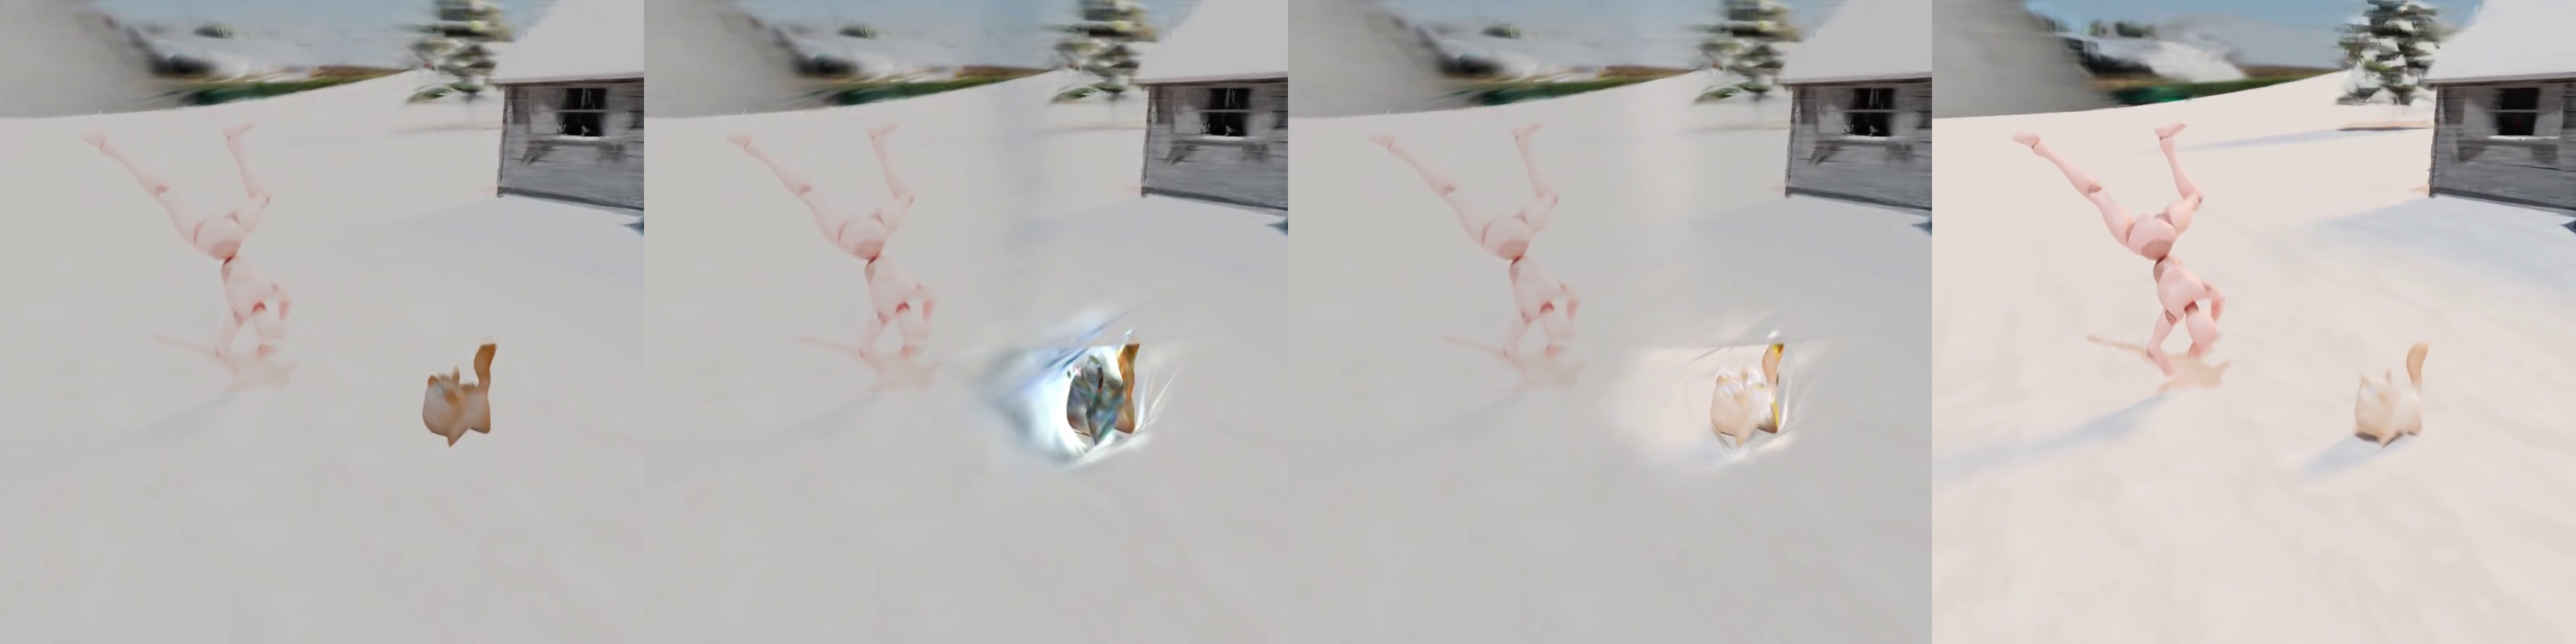
\includegraphics[width=\textwidth]{figures/transsplat_comparison.png}
\caption{Static scene comparison (same viewpoint). From left to right: (1)~Original Scene A with mismatched cat lighting, (2)~TranSplat closed-form SH transfer, which introduces a blue/grey halo around the cat, (3)~our DC-only SH optimization, which produces a clean color shift, (4)~Scene B ground truth. TranSplat degrades quality because 4DGS SH coefficients entangle material and lighting, violating TranSplat's factorization assumption.}
\label{fig:transsplat}
\end{figure*}

\paragraph{Dynamic Scene Results.}
Table~\ref{tab:dynamic_results} compares SH band optimization strategies on the dynamic scene with an animated breakdancer. All methods use Scene B renders as optimization targets (500 iterations). The table measures reconstruction fidelity against Scene A (i.e., how much each method alters the original scene). All harmonization methods necessarily reduce Scene A fidelity since they modify the object's appearance, but DC-only optimization causes the least degradation while producing the cleanest visual result. All-band optimization causes the most degradation (PSNR drops from 19.22 to 17.59) and introduces severe rainbow artifacts visible in Figure~\ref{fig:dynamic_comparison}, as the optimizer overfits view-dependent SH terms to match training views at the expense of novel-view consistency.

\begin{table}[t]
\centering
\small
\begin{tabular}{lccc}
\toprule
Method & PSNR $\uparrow$ & SSIM $\uparrow$ & LPIPS $\downarrow$ \\
\midrule
Original A & 19.22 & 0.8915 & 0.183 \\
All-band ($\text{lr}=0.01$) & 17.59 & 0.8697 & 0.262 \\
Band regularization & 17.69 & 0.8809 & 0.234 \\
Separate LR & 17.77 & 0.8834 & 0.221 \\
\textbf{DC-only} & \textbf{17.77} & \textbf{0.8831} & \textbf{0.221} \\
\bottomrule
\end{tabular}
\caption{Dynamic Blender scene with different SH optimization strategies, measured against Scene A reconstruction quality. All methods reduce fidelity (expected, since they modify the object's appearance), but DC-only preserves the most while producing clean relighting. All-band optimization causes the largest degradation and introduces rainbow artifacts (Figure~\ref{fig:dynamic_comparison}).}
\label{tab:dynamic_results}
\end{table}

\begin{figure*}[t]
\centering
\begin{subfigure}{0.24\textwidth}
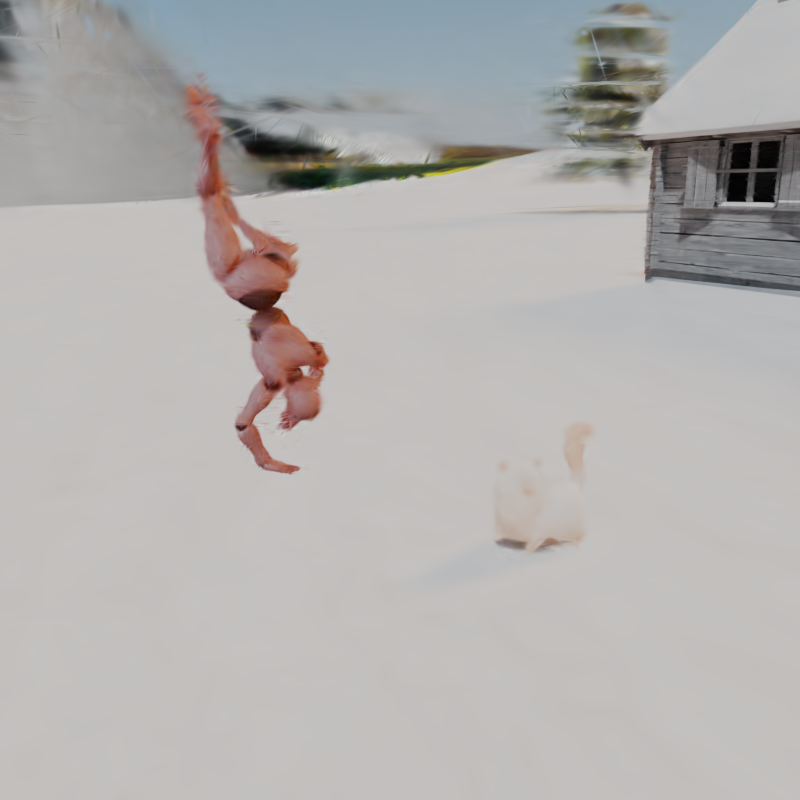
\includegraphics[width=\linewidth]{figures/v5_original.png}
\caption{Original (dark)}
\end{subfigure}
\hfill
\begin{subfigure}{0.24\textwidth}
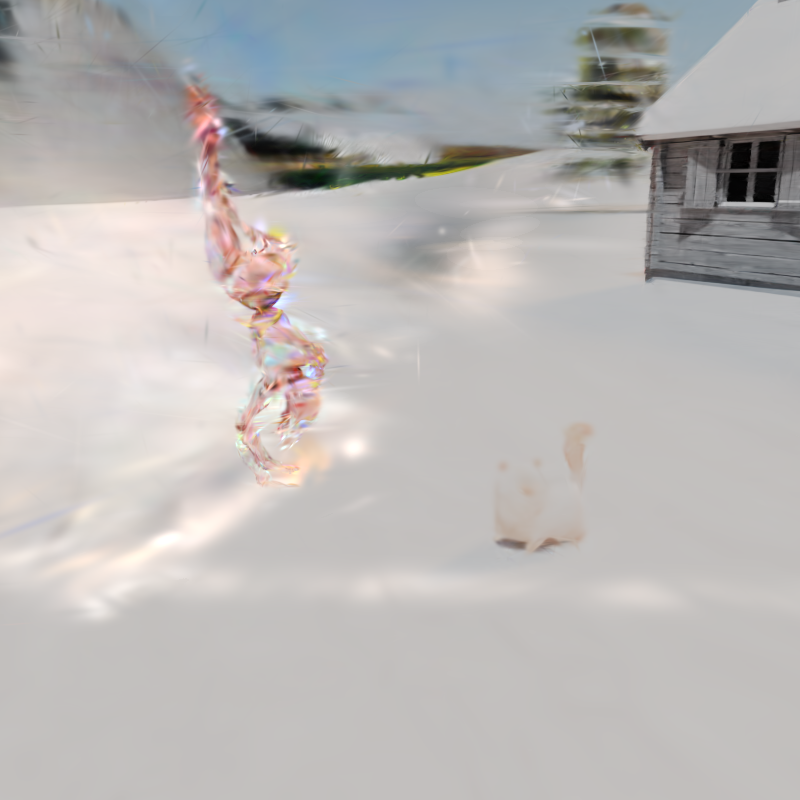
\includegraphics[width=\linewidth]{figures/v5_allband.png}
\caption{All-band (rainbow)}
\end{subfigure}
\hfill
\begin{subfigure}{0.24\textwidth}
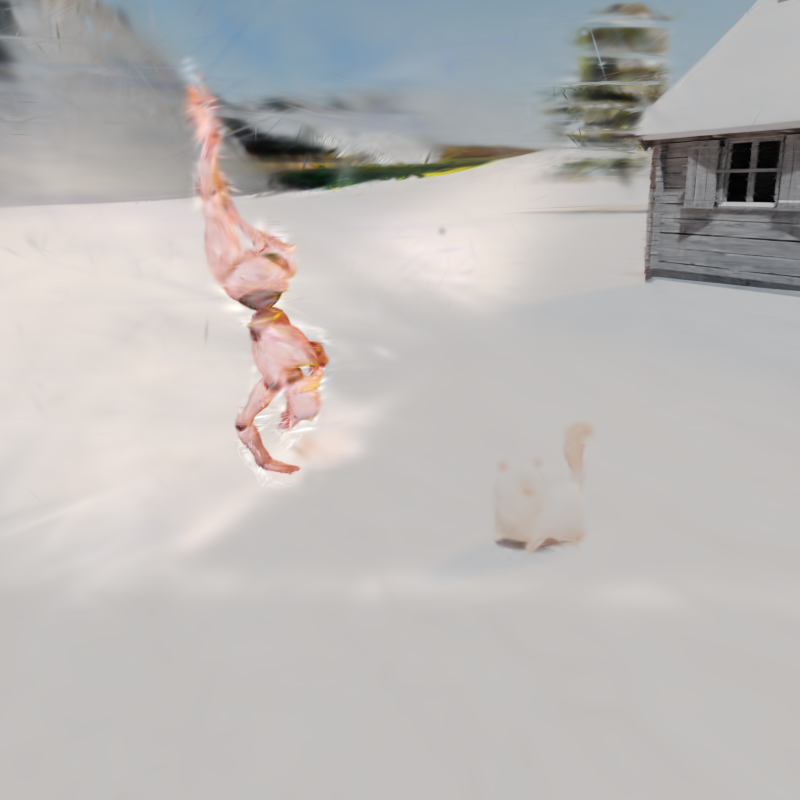
\includegraphics[width=\linewidth]{figures/v5_dc_only.png}
\caption{DC-only (ours)}
\end{subfigure}
\hfill
\begin{subfigure}{0.24\textwidth}
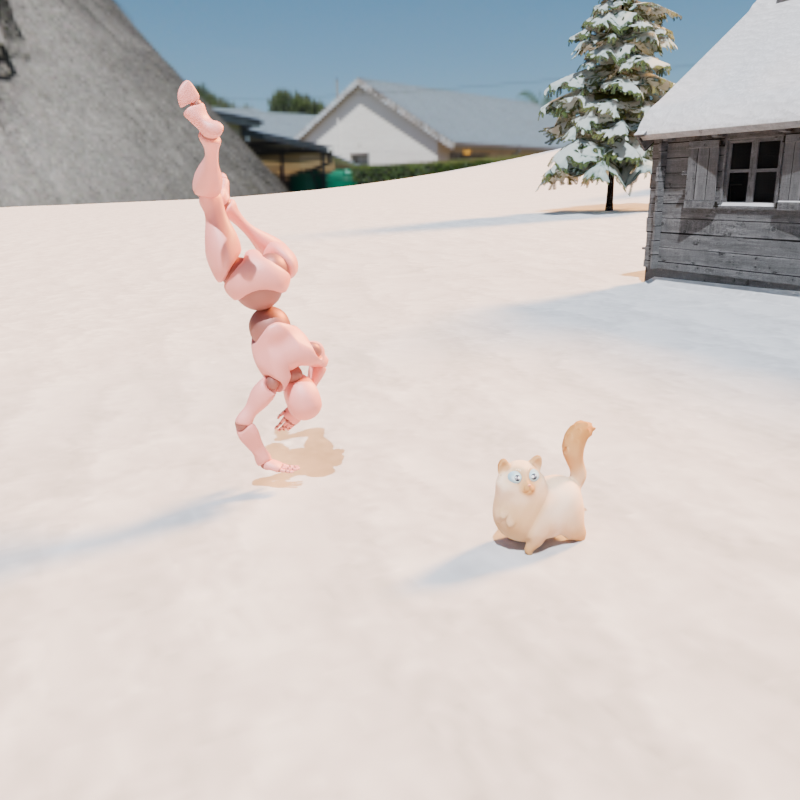
\includegraphics[width=\linewidth]{figures/v5_ground_truth.png}
\caption{Ground truth (full re-lit)}
\end{subfigure}
\caption{Dynamic scene relighting comparison. (a) The original breakdancer appears too dark and red. (b) All-band SH optimization produces severe rainbow/iridescent artifacts despite improving pixel-level metrics at training views. (c) DC-only optimization achieves a clean brightness shift without view-dependent artifacts. (d) Ground truth rendering under target lighting.}
\label{fig:dynamic_comparison}
\end{figure*}

\subsection{Real-World HyperNeRF Scene}

As a complementary experiment, we composite a chocolate bar (segmented from a separate capture) onto the cutting board of a HyperNeRF~\cite{park2021hypernerf} cookie scene from the SA4D~\cite{ji2024segment4dgaussians} dataset. The raw composite contains visible seams and rendering artifacts around the inserted object.

From there, we run our gradient-based harmonization pipeline on the scene. For this real capture we use the Whitebox Harmonizer~\cite{ke2022harmonizer} as the target generator. Using real-life HyperNeRF data makes masking a much larger issue compared with Blender, as the SA4D-derived Gaussian mask must be projected through a dynamic, semi-transparent splat renderer: boundaries are soft, coverage shifts as the scene deforms, and small mask errors leak background into the object (or vice versa), which directly leads to halos and unstable SH updates. Because this scene has no paired relighting ground truth, targets come from the 2D harmonizer applied per frame, so supervision can vary over time even when the underlying geometry is coherent. Together with imperfect projected masks, that makes high-order SH easy to overfit, which matches what we observe on synthetic data. As a result, keeping updates on the DC band only tends to give more stable results.

We attempt to improve the remaining rendering artifacts by running DiFix~\cite{difix3d2024}, a single-step 2D diffusion fixer that is one component of the full DiFix3D+ static-3DGS refinement pipeline. We apply DiFix per rendered frame and re-encode as video: this is purely 2D, does not alter Gaussians, and therefore preserves 4D motion. We do not run the full DiFix3D+ trainer, which re-optimizes a static splat and would conflict with or erase our time-varying 4DGS composite.

Figure~\ref{fig:difix_results} shows the results. DiFix reduces compositing seams around the inserted chocolate and sharpens the overall render. However, because each frame is processed independently, corrections can differ across frames and are not 3D-consistent. We also attempted to use the DiFix frame outputs as optimization targets to distill corrections back into SH coefficients, but the per-frame inconsistencies in the DiFix outputs meant the resulting 3D model lost temporal motion and produced a static result.

We also experimented with procedural shadow injection using dark, low-opacity Gaussians placed beneath the inserted object via plane projection, which adds visual grounding (Figure~\ref{fig:shadow}). In still frames this reduces a ``floating object'' look, but it is not a physical lighting model. Shadow extent, softness, and opacity are hand-tuned and can appear as smudges or dark spots once the insert is harmonized. A static shadow patch also misaligns under temporal deformation unless refit each frame.

\begin{figure}[t]
\centering
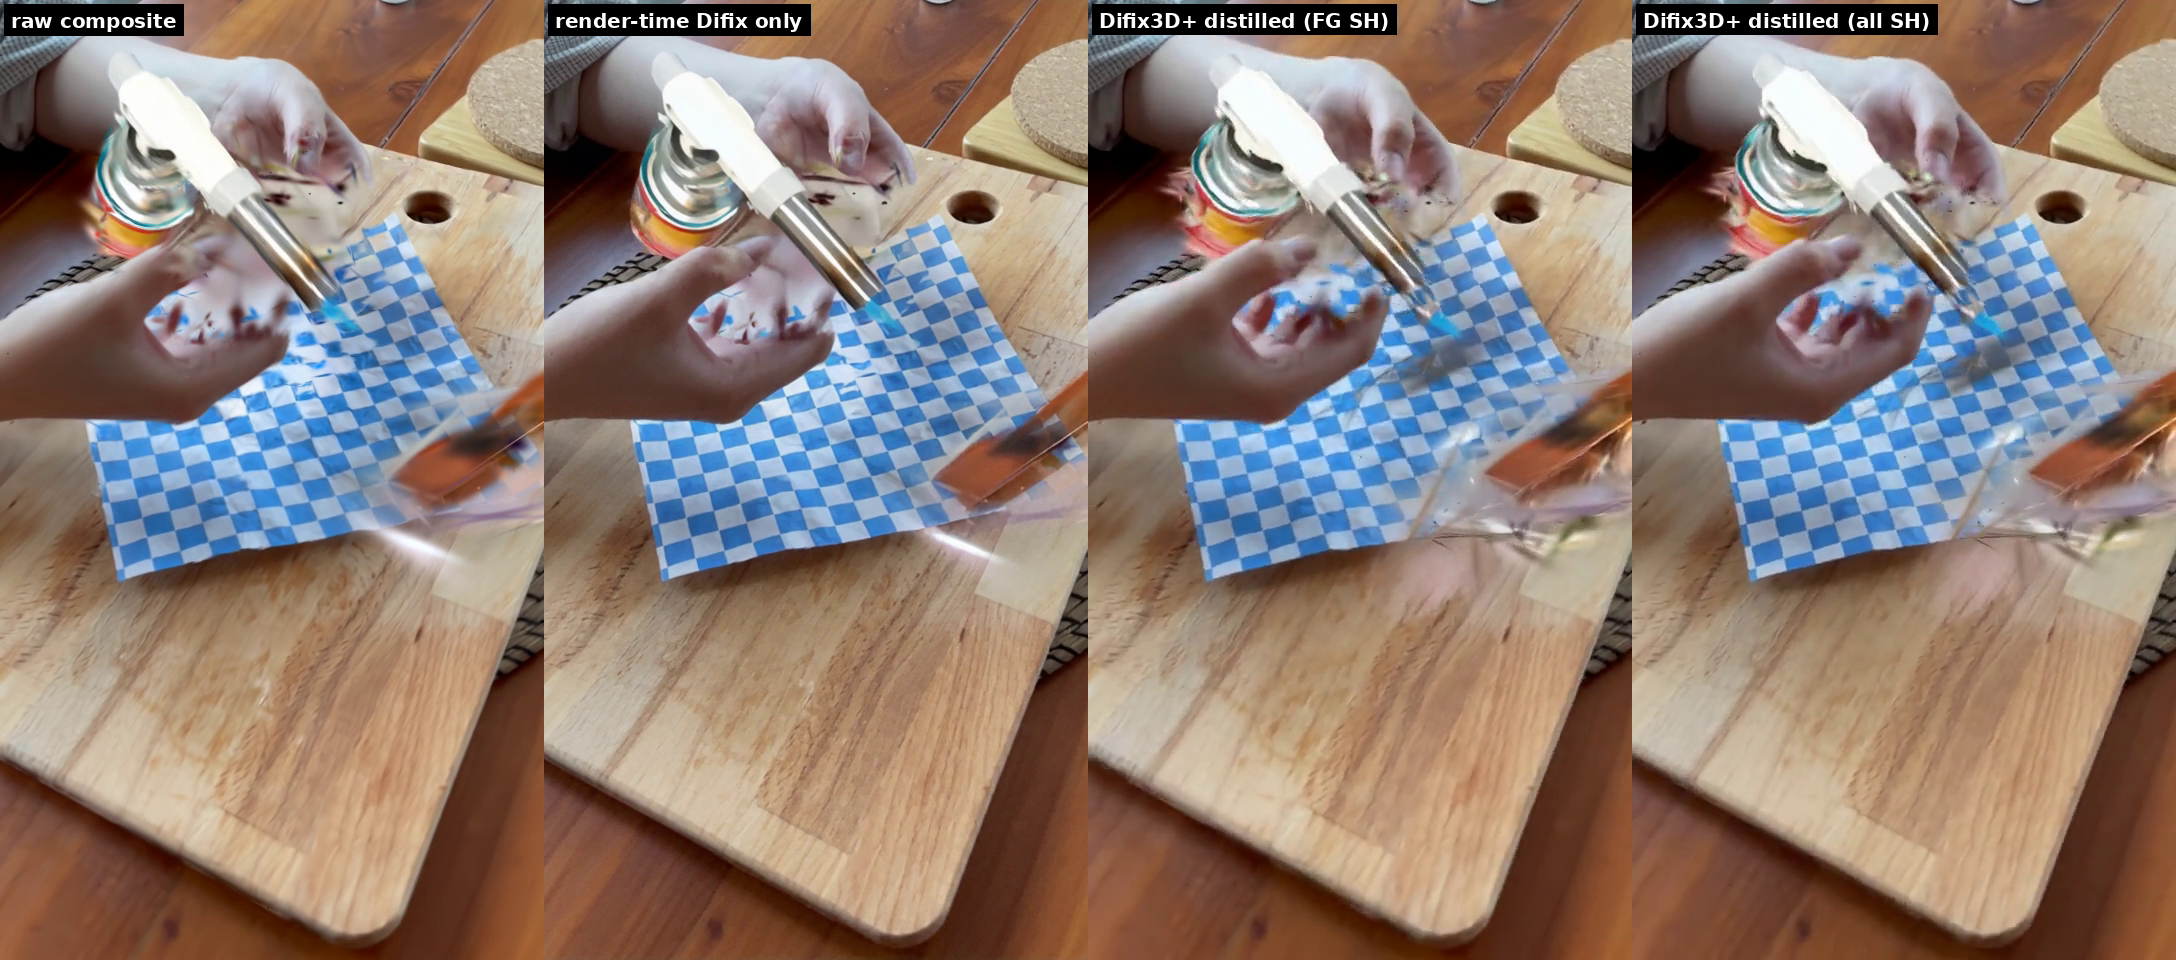
\includegraphics[width=\linewidth]{figures/difix3d_preview.png}
\caption{HyperNeRF cookie scene with composited chocolate. Left to right: raw composite, DiFix cleaned per-frame, and two variants where DiFix outputs were used as SH optimization targets (foreground only, all Gaussians). The per-frame DiFix cleanup reduces compositing seams but the SH distillation attempts did not preserve temporal motion.}
\label{fig:difix_results}
\end{figure}

\begin{figure}[t]
\centering
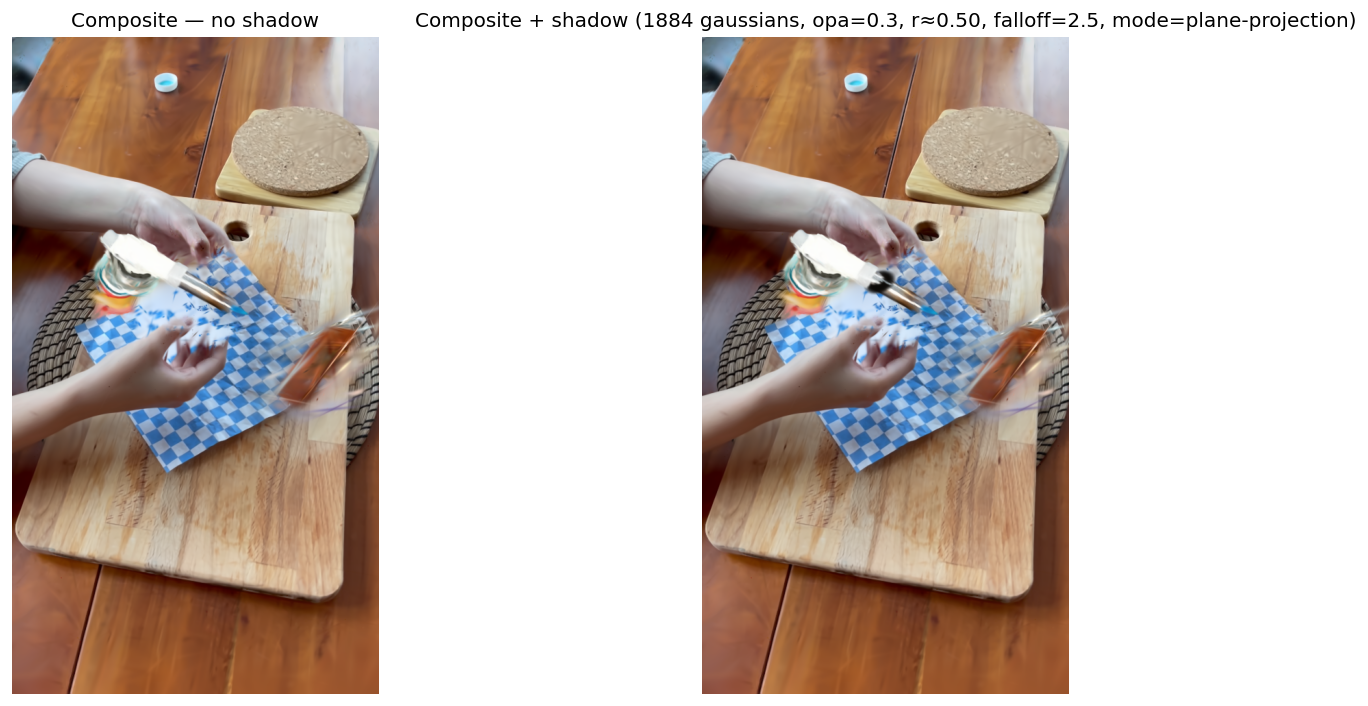
\includegraphics[width=\linewidth]{figures/shadow_compare.png}
\caption{Procedural shadow injection. Left: composite without shadow. Right: composite with plane-projected shadow Gaussians (1884 Gaussians, opacity 0.3). The shadow adds visual grounding for the inserted object.}
\label{fig:shadow}
\end{figure}

%%%%%%%%% DISCUSSION
\section{Discussion}

\paragraph{Why DC-Only Works.}
The effectiveness of DC-only optimization can be understood through the structure of the SH basis. The DC coefficient ($Y_0^0$) represents uniform, view-independent radiance. Relighting an object from one environment to another primarily changes the overall brightness and color temperature, both of which are captured by DC. Higher-order SH bands ($l \geq 1$) encode view-dependent effects like specular highlights and color gradients across the surface. When the optimizer modifies these bands, it can match training-view pixels exactly but creates color patterns that are inconsistent across viewpoints. This is analogous to overfitting in traditional machine learning: the model explains training data well but generalizes poorly.

\paragraph{Limitations of the Approach.}
Our method has several limitations. First, DC-only optimization can only apply a uniform color shift per Gaussian, so it cannot capture view-dependent lighting differences between source and target environments (e.g., specular highlights that move with viewpoint). Second, the quality of harmonization depends entirely on the target generation method: harmonizer CNNs can produce temporally inconsistent targets, and DiFix occasionally hallucinates details. Third, the 2D mask projection from 3D Gaussian masks is approximate, particularly for semi-transparent Gaussians and dynamic scenes where deformation changes mask coverage over time. We found that a very low binarization threshold (0.01 instead of the standard 0.5) was necessary to achieve adequate mask coverage.

\paragraph{TranSplat Failure Analysis.}
TranSplat assumes that a Gaussian's SH coefficients can be factored as $\text{SH}_{\text{stored}} = \text{BRDF} \times \text{Lighting}_{\text{source}}$, allowing relighting via the ratio $\text{Lighting}_{\text{target}} / \text{Lighting}_{\text{source}}$. In 4DGS, this factorization fails because SH coefficients absorb not just lighting but also material albedo, geometric compensation (Gaussians use SH to explain appearance that their covariance cannot), and deformation residuals. Applying TranSplat's lighting ratio therefore corrupts rather than corrects the appearance. Additionally, TranSplat's quasi-random environment map sampling with 1200 directions has a 96\% probability of completely missing concentrated light sources like the sun, producing incorrect SH transfer ratios.

\paragraph{Comparison to 2D Harmonization.}
A natural alternative to our 3D SH optimization is to simply run a 2D harmonizer on each rendered frame independently. This approach works for fixed viewpoint videos but fails for interactive applications where users can change the camera freely, because 2D harmonization is not 3D-consistent. Our method optimizes the underlying 3D representation, ensuring that corrections remain consistent across arbitrary viewpoints and timesteps.

\paragraph{IC-Light: Diffusion-Based Relighting.}
We also evaluated IC-Light, a diffusion-based relighting model that takes a foreground object and background image and generates a relit version of the foreground to match the background illumination. On the dynamic Blender scene, IC-Light achieves 20.73 dB PSNR against the Scene B ground truth, surpassing our DC-only method (19.63 dB on the same scene) in per-pixel color accuracy. However, because IC-Light runs a full diffusion process independently per frame, it produces severe temporal flickering: object shape, texture, and fine details change from frame to frame. Figure~\ref{fig:iclight} shows two frames from the same video where the cat's shape and the breakdancer's limbs are generated differently despite identical 3D content. This inconsistency makes IC-Light unsuitable as a target generator for 3D SH distillation, since conflicting per-frame targets would produce incoherent SH updates. Our optimization-based approach trades per-frame color accuracy for 3D and temporal consistency, which is the fundamental requirement for interactive novel-view applications.

\begin{figure}[t]
\centering
\begin{subfigure}{\linewidth}
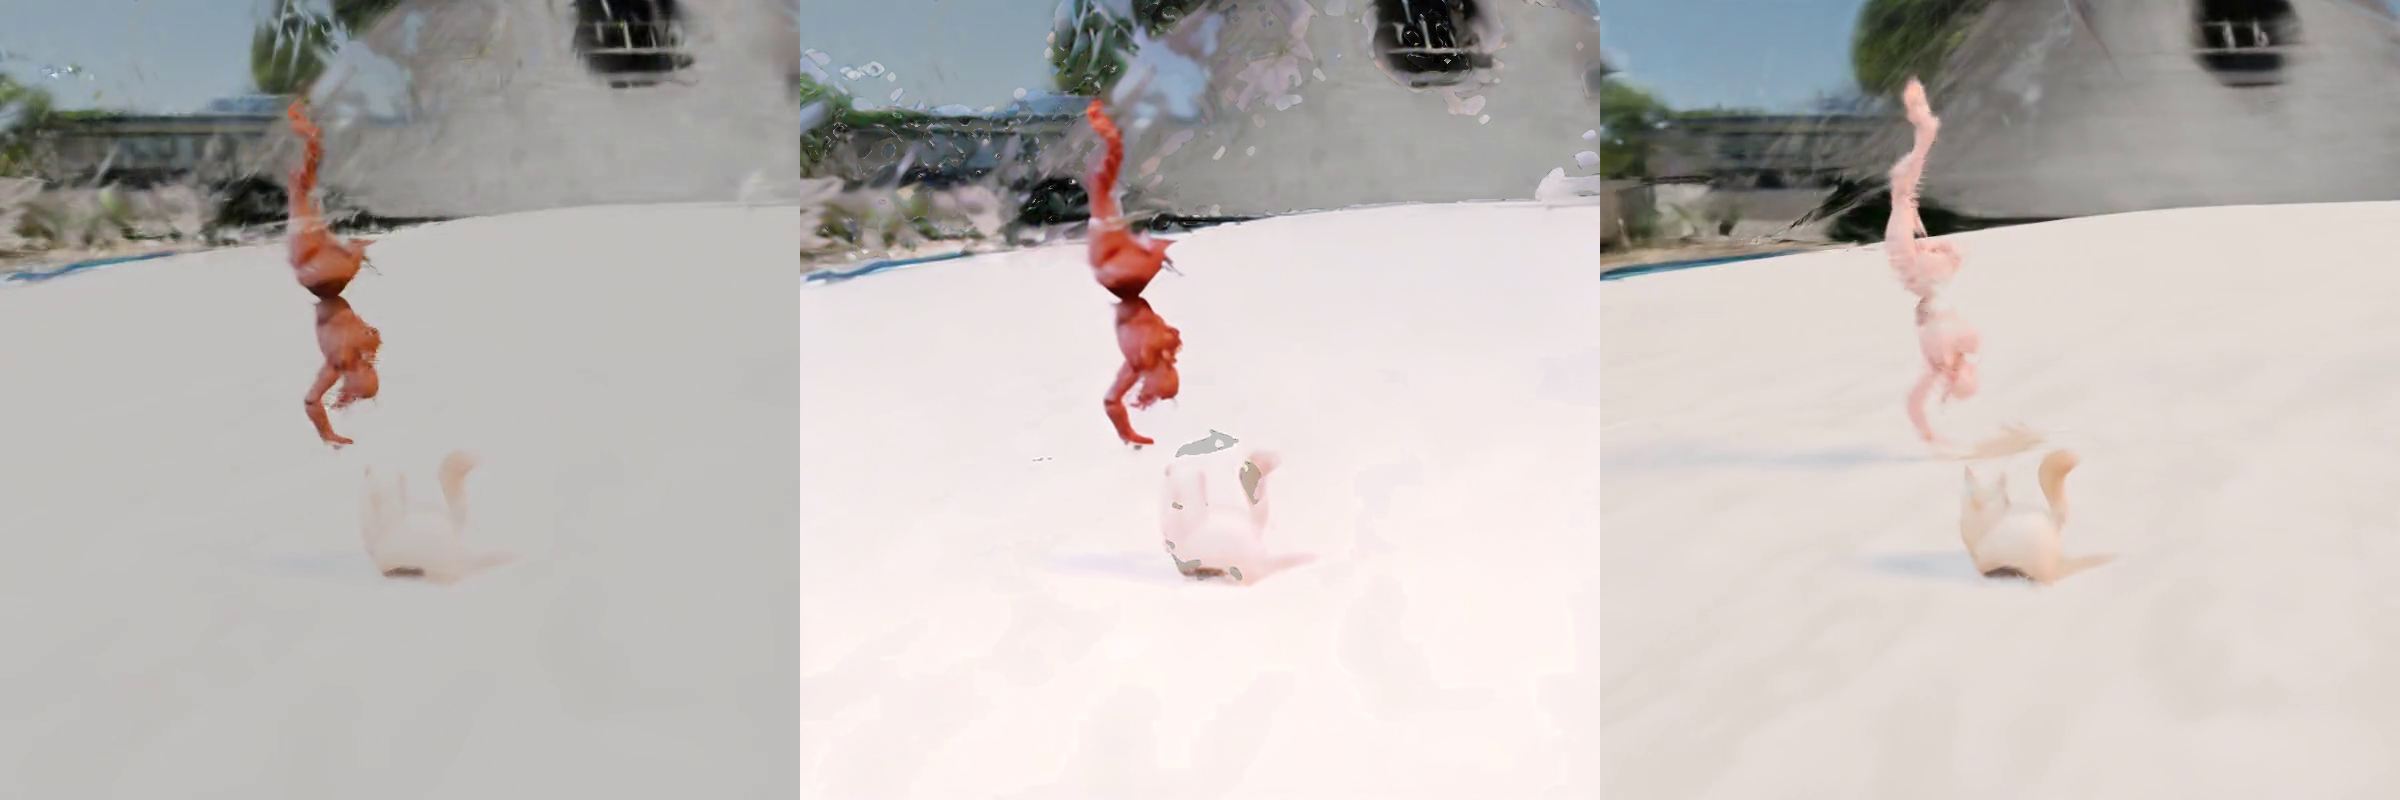
\includegraphics[width=\linewidth]{figures/iclight_frame05.png}
\caption{Frame 5}
\end{subfigure}
\vspace{2pt}
\begin{subfigure}{\linewidth}
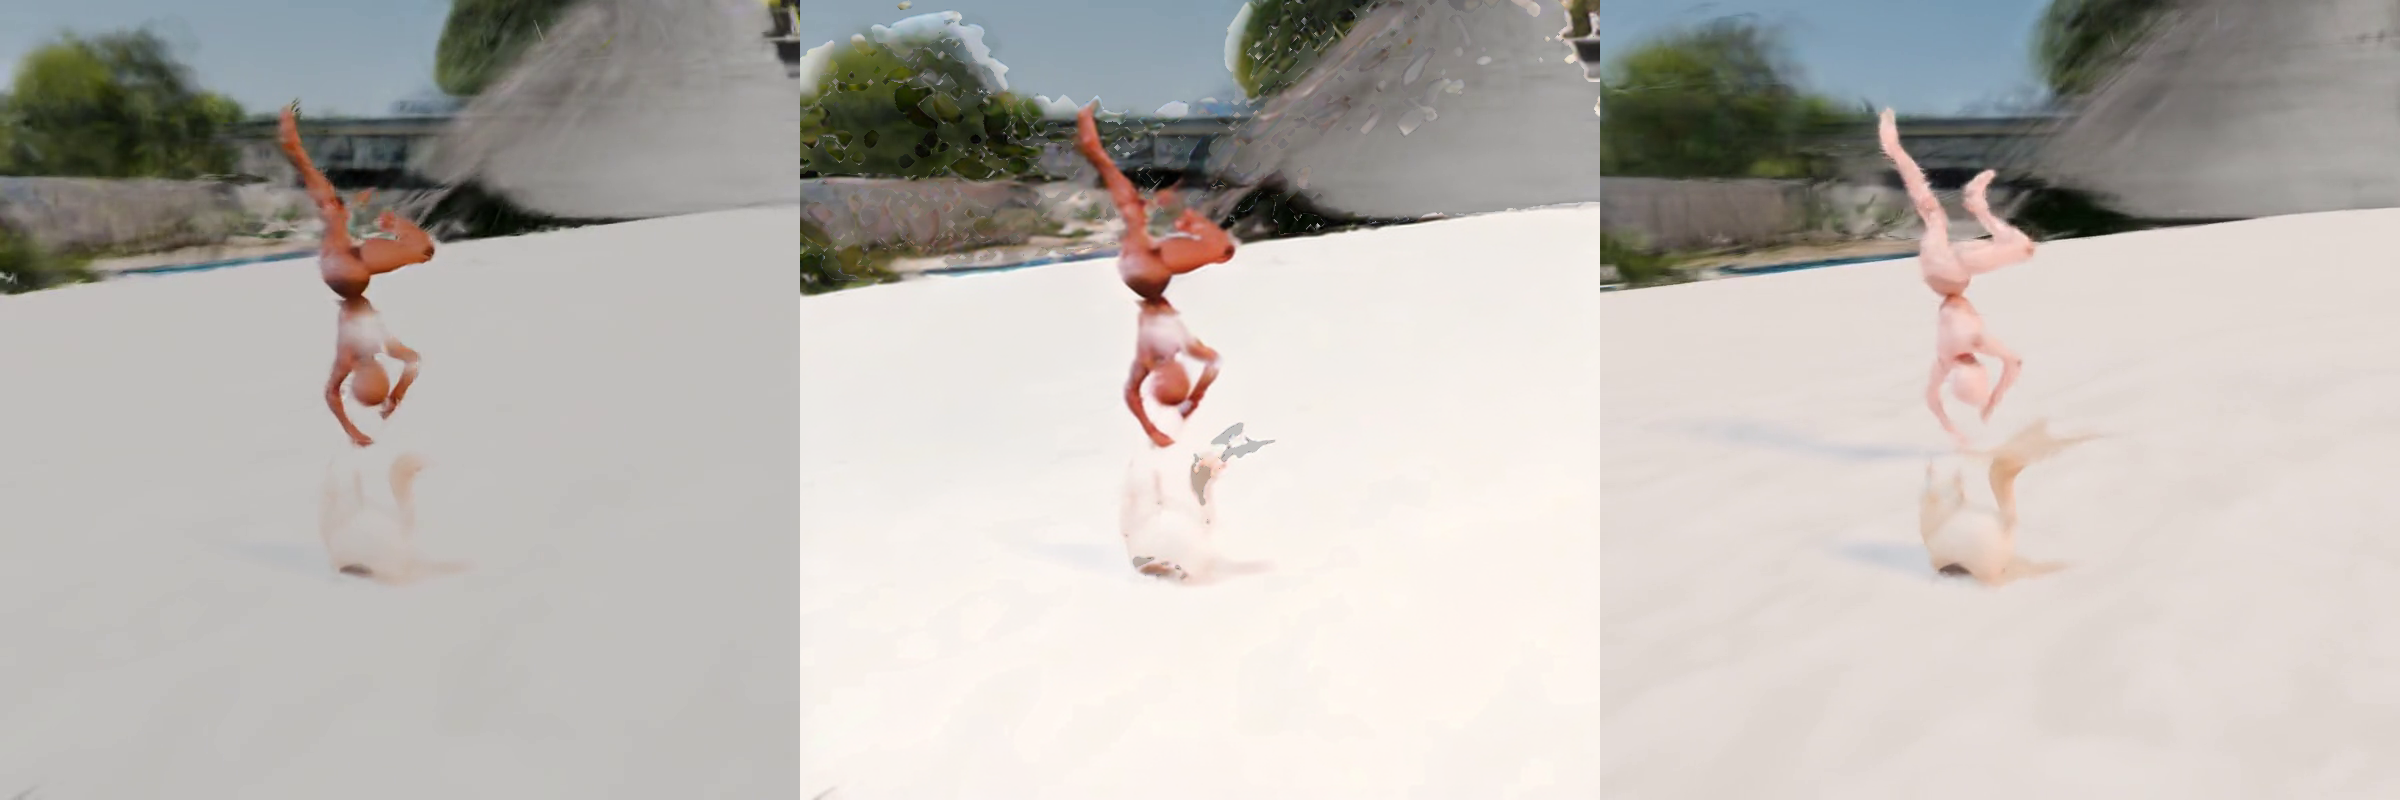
\includegraphics[width=\linewidth]{figures/iclight_frame15.png}
\caption{Frame 15}
\end{subfigure}
\caption{IC-Light relighting on two frames from the same video. Each row shows: original Scene A (left), IC-Light output (center), Scene B ground truth (right). While IC-Light shifts the breakdancer's color closer to ground truth, the cat's shape and background details change between frames due to the stochastic diffusion process, producing temporal flickering.}
\label{fig:iclight}
\end{figure}

%%%%%%%%% CONCLUSION
\section{Conclusion}

We presented a pipeline for harmonizing composite objects in 4D Gaussian Splatting scenes through gradient-based SH coefficient optimization. By restricting updates to the DC SH band, our method achieves clean relighting without the rainbow artifacts that arise from full-band optimization. On a custom Blender benchmark with controlled lighting, our approach outperforms TranSplat's closed-form SH transfer by 1.1 dB PSNR. We additionally explored using DiFix3D+ for per-frame artifact cleanup on real-world HyperNeRF composites, finding that while it improves individual frame quality, its per-frame inconsistencies prevent it from serving as a stable optimization target for 3D SH distillation. Our benchmark and pipeline code are publicly available.

Future work could explore jointly optimizing DC and a small number of higher-order coefficients with strong regularization to capture subtle view-dependent lighting effects without rainbow artifacts. Incorporating physics-based priors (estimated environment maps, approximate BRDF) could also improve relighting quality beyond what pure data-driven optimization achieves.

\section*{Supplementary Videos}

Video results for all experiments are available at the following links. All videos are hosted on Google Drive.

\begin{itemize}
\item \textbf{4DGS DC-only harmonized}: \url{https://drive.google.com/drive/u/1/folders/1mmNakvQiGdgMoSbHZh-_OSMlGDVYOyrm}
\item \textbf{4DGS all-band harmonized}: \url{https://drive.google.com/drive/u/1/folders/1mmNakvQiGdgMoSbHZh-_OSMlGDVYOyrm}
\item \textbf{4DGS unharmonized}: \url{https://drive.google.com/drive/u/1/folders/1mmNakvQiGdgMoSbHZh-_OSMlGDVYOyrm}
\item \textbf{TranSplat scene}: \url{https://drive.google.com/drive/u/1/folders/1mmNakvQiGdgMoSbHZh-_OSMlGDVYOyrm}
\item \textbf{3DGS unharmonized}: \url{https://drive.google.com/drive/u/1/folders/1mmNakvQiGdgMoSbHZh-_OSMlGDVYOyrm}
\item \textbf{3DGS harmonized}: \url{https://drive.google.com/drive/u/1/folders/1mmNakvQiGdgMoSbHZh-_OSMlGDVYOyrm}
\item \textbf{3DGS ground truth}: \url{https://drive.google.com/drive/u/1/folders/1mmNakvQiGdgMoSbHZh-_OSMlGDVYOyrm}
\item \textbf{All assets}: \url{https://drive.google.com/drive/u/1/folders/1mmNakvQiGdgMoSbHZh-_OSMlGDVYOyrm}
\end{itemize}

We used AI to assist us in generating this paper.

{\small
\bibliographystyle{ieee_fullname}
\bibliography{egbib}
}

\end{document}
